%%%--------------------------------%%%
%%% UC10
%%%--------------------------------%%%

\newpage
% UC10 ====================================================
\subsubsection{Use Case Specification: \ac{UC}10 Activity Stream}
\label{sec:domainBbk}

\paragraph*{Description}\mbox{}\\
A user should be able to see the latest activity (see chapter \ref{sec:theoryBc}) in the given enviroment.


\paragraph*{Basic Flow} \mbox{}\\
\noindent
Activity Stream: 
\begin{itemize}
	\vspace{-3mm}
	\setlength\itemsep{-1em}
	\item The user opens the home page where the activity stream can be found.
	\item Within the activity stream the user can then find the latest activities (examples mentioned above).
	\item Depending on the activity the user has the chance to interact with it and will be redirected to the specific item (e.g. a user can click on a new risks shown in his activity stream to open it).
\end{itemize} 
\\
\begin{figure}[H]
	\centering
	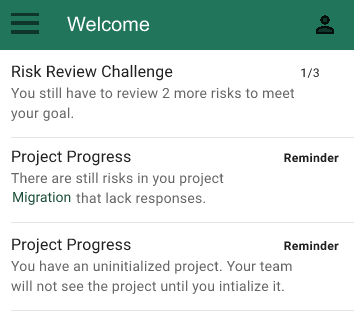
\includegraphics[width=0.3\textwidth]{Assets/UC_Screenshots/UC10S.png}
	\caption{Use Case 10: Mock Prototype}
	\label{fig:useCase10Detail}
\end{figure}
\newpage
\subparagraph{Activity Diagram}\mbox{}\\
\begin{figure}[H]
	\centering
	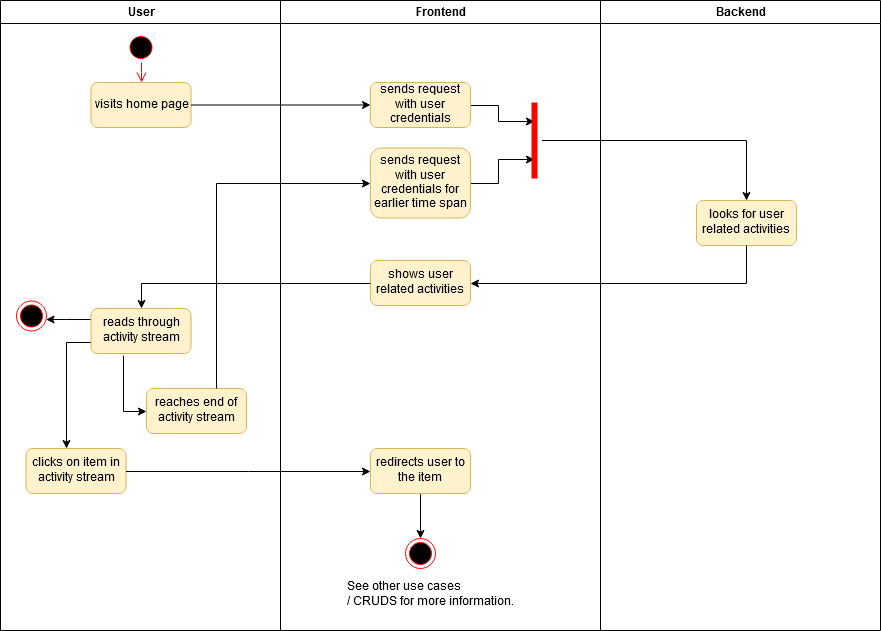
\includegraphics[width=0.8\textwidth]{Content/Domain/UC10ActivityStream.png}
	\caption{Activity Diagram \ac{UC}10 Activity Stream}
	\label{fig:label11}
\end{figure}

\paragraph*{Special Requirements and Preconditions}\mbox{}\\
As the activity contains personalized information, the following preconditions have to be fulfilled.
\begin{enumerate}
	\vspace{-3mm}
	\setlength\itemsep{-1em}
	\item The user has to be logged in.
	\item Alternatively a visitor can login to be redirect to the personal home page.
\end{enumerate}

